\documentclass[lettersize,journal]{IEEEtran}

% ═══════════════════════ PACKAGES ═══════════════════════
\usepackage[T1]{fontenc}
\usepackage[utf8]{inputenc}
\usepackage{amsmath,amssymb,amsfonts}
\usepackage{amsthm}
\usepackage{bm}

% ── Theorem-like environments ───────────────────────────────────────────
\newtheorem{theorem}{Theorem}
\newtheorem{proposition}{Proposition}
\newtheorem{lemma}{Lemma}
\newtheorem{corollary}{Corollary}
\theoremstyle{definition}
\newtheorem{definition}{Definition}
\newtheorem{assumption}{Assumption}
\theoremstyle{remark}
\newtheorem{remark}{Remark}
\usepackage{graphicx}
\usepackage{cite}
\usepackage{algorithmic}
\usepackage{algorithm}
\usepackage{url}
\usepackage{hyperref}
\usepackage{color}
\usepackage{booktabs}
\usepackage{multirow}
\usepackage{subcaption}
\usepackage{siunitx}
\usepackage{tikz}
\usepackage{stfloats}
\usepackage{array}
\usepackage{textcomp}
\usepackage{verbatim}
\usetikzlibrary{arrows.meta,positioning,calc}
\hyphenation{op-tical net-works semi-conduc-tor IEEE-Xplore}

% ═══════════════════════ MATH COMMANDS ═══════════════════
\newcommand{\R}{\mathbb{R}}
\newcommand{\norm}[1]{\left\| #1 \right\|}
\newcommand{\vect}[1]{\bm{#1}}
\newcommand{\mat}[1]{\mathbf{#1}}
\newcommand{\dt}{\Delta t}
\newcommand{\st}{\text{s.t.}}

% Safe set barrier function shorthand
\newcommand{\hcbf}{h}          % barrier function h(x)
\newcommand{\xcbf}{\vect{x}}   % state
\newcommand{\ucbf}{\vect{u}}   % control input

% ═══════════════════════════════════════════════════════════

\begin{document}

\title{Safety-Critical Evasion for Quadrotor UAVs:\\
       NMPC with Embedded High-Order Control Barrier Functions\\
       Against an Adversarial Pursuer}

\author{Bryan~S.~Guevara,
        Luis~F.~Simancas,
        and~Tiago~Nascimento%

\thanks{Manuscript received April 2025.}%
\thanks{Bryan~S.~Guevara is with the Laboratório de Automação
        e Sistemas de Robótica (LaSER), Universidade Federal da
        Paraíba (UFPB), João Pessoa, PB 58051-900, Brazil.
        {\tt\small bguevara@laser.ufpb.br}}%
\thanks{Luis~F.~Simancas is with Instituto de Automática (INAUT),
        Universidad Nacional de San Juan--CONICET, Argentina.
        {\tt\small lsimancas@inaut.unsj.edu.ar}}%
\thanks{Tiago~Nascimento is with the Laboratório de Automação
        e Sistemas de Robótica (LaSER), Universidade Federal da
        Paraíba (UFPB), João Pessoa, PB 58051-900, Brazil.
        {\tt\small tiago@laser.ufpb.br}}%
}

\markboth{IEEE Robotics and Automation Letters}%
{Guevara \MakeLowercase{\textit{et al.}}:
 Safety-Critical Evasion via NMPC-HOCBF for Quadrotors}

\IEEEpubid{0000--0000/00\$00.00~\copyright~2025 IEEE}

\maketitle

% ═══════════════════════ ABSTRACT ════════════════════════
\begin{abstract}
This paper addresses the one-vs-one aerial pursuit-evasion problem
for quadrotor UAVs operating in a \emph{bounded workspace}.
We propose a Nonlinear Model Predictive Control (NMPC) framework for
the evader in which two safety constraints are enforced simultaneously
as \emph{hard-constraint degree-2 High-Order Control Barrier Functions}
(HOCBFs) embedded inside the Optimal Control Problem (OCP):
(i)~a minimum-separation barrier preventing capture, and
(ii)~a workspace-containment barrier bounding the flight volume.
The two barriers have competing objectives near the workspace boundary
under aggressive pursuit---the \emph{cornering} scenario that makes
post-hoc CBF-QP filters infeasible or generates chattering---and the
receding-horizon optimizer resolves them jointly without explicit
priority rules.
The pursuer is modeled as an augmented constant-velocity state in the
OCP, providing multi-step foresight over both barrier boundaries.
Both barriers are shown to have relative degree~2 from the collective
thrust $T$, yielding affine HOCBF conditions encoded as nonlinear
stage constraints in acados with SQP-RTI.
Both agents run independent solvers at \SI{100}{\hertz}
(decoupled game architecture).
Software-in-the-Loop experiments in MuJoCo with two full quadrotor
models validate: (a)~zero constraint violations including deliberate
cornering scenarios where the pursuer drives the evader against the
workspace boundary; (b)~superiority over a post-hoc CBF-QP filter,
which accumulates safety violations and physical collisions under the
same conditions; and (c)~real-time feasibility within a
\SI{3}{\milli\second} budget at \SI{100}{\hertz}.
\end{abstract}

\begin{IEEEkeywords}
Pursuit-Evasion, Control Barrier Functions, Nonlinear Model Predictive
Control, Quadrotor UAV, Adversarial Games, Workspace Constraints,
Safety-Critical Control, acados.
\end{IEEEkeywords}

\IEEEpubidadjcol

% ═══════════════════════ I. INTRODUCTION ═════════════════
\section{Introduction}
\label{sec:intro}

\IEEEPARstart{A}{dversarial} scenarios involving autonomous aerial
vehicles have attracted increasing attention as unmanned aerial
systems (UAS) are deployed in competitive or contested
environments~\cite{mueller2015model, mellinger2011minimum}.
The one-vs-one aerial pursuit-evasion game---where a pursuer attempts
to minimize its distance to an evader while the evader strives to
maximize it---is a canonical instance of a zero-sum differential
game~\cite{isaacs1965differential} that captures the essential
tension between aggressive maneuvering and safety-critical separation
guarantees.
Beyond academic interest, the problem is directly relevant to
counter-drone systems, autonomous air combat, and multi-agent
coordination under adversarial conditions~\cite{shaferman2008cooperative}.

\subsection{Existing Approaches and Their Limitations}

\subsubsection{Reinforcement Learning Dominance}
The dominant paradigm in recent drone pursuit-evasion literature is
multi-agent reinforcement learning (MARL).
Wang \emph{et al.}~\cite{wang2022game} proposed an online
planning framework using deep RL for multi-UAV pursuit-evasion,
demonstrating emergent cooperative strategies.
Subsequent works have advanced this direction with asynchronous
multi-stage adversarial training~\cite{gu2024learning},
population-based self-play and adaptive teaming in real
CrazyFlie deployments~\cite{lin2025adaptive}, and
zero-shot sim-to-real transfer on three quadrotors with
body-rate-level commands~\cite{zhang2024online}.
The 2025 work by Kaufmann \emph{et al.}~\cite{kaufmann2025learned}
further demonstrates that body-rate control enables significantly more
agile evasion compared to velocity-level commands.

Despite these advances, RL-based approaches share a fundamental
limitation: they provide no \emph{formal guarantees} on constraint
satisfaction.
A learned policy may violate minimum separation requirements during
exploration, generalize poorly to unseen adversary behaviors,
and offers no certificate of forward invariance of the safe set.
This gap is particularly critical in safety-certified airspace or
in scenarios where physical contact implies mission failure.

\subsubsection{Model Predictive Control Approaches}
Model Predictive Control (MPC) provides a principled alternative
that admits explicit constraint encoding and offers receding-horizon
optimality guarantees.
Early applications to pursuit-evasion treated the problem as a
non-cooperative MPC game, where Selvakumar and
Bakolas~\cite{selvakumar2021pursuit} compared game-theoretic planners
with naive MPC on simplified agents, showing that anticipating the
opponent's strategy is essential.
More recently, Belinha~\emph{et al.}~\cite{belinha2024noncooperative}
formulated a non-cooperative MPC for capturing a remotely piloted
drone, but restricted the MPC to the pursuer only, using a heuristic
evasion policy and simplified 3-DOF kinematics.
The most closely related work,~\cite{zhan2025nonlinear}, extends
standard NMPC to a minimax receding-horizon differential game for
drone racing---demonstrating that a game-aware formulation outperforms
a standard NMPC pursuer---but addresses a racing (not evasion)
objective, operates in simulation only, and does not provide
formal safety guarantees for the evader.

A parallel line of work addresses decentralized NMPC for
\emph{cooperative} multi-quadrotor systems~\cite{zeng2024decentralized},
where pairwise safety constraints are handled within the MPC horizon.
However, the cooperative setting imposes symmetric information and
aligned objectives; in a pursuit-evasion game, the pursuer actively
seeks to violate the evader's safety constraint, and the safe set
boundary moves in a hostile direction across the prediction horizon.
No prior work addresses this adversarial moving-boundary feasibility
challenge in an NMPC framework.

\subsubsection{Control Barrier Functions as Post-Hoc Safety Filters}
Control Barrier Functions (CBFs), introduced by
Ames~\emph{et al.}~\cite{ames2019control}, provide forward-invariance
guarantees for a safe set $\mathcal{C} = \{x : h(x) \geq 0\}$ by
enforcing $\dot{h}(x,u) \geq -\gamma\,h(x)$ for a class-$\mathcal{K}$
function $\gamma$.
The CBF condition is commonly imposed as a Quadratic Program (CBF-QP)
that minimally modifies a nominal control input to satisfy
safety~\cite{ames2019control}.
In multi-UAV pursuit-evasion, this architecture has been applied
to prevent inter-agent collisions among
fixed-wing pursuers~\cite{chu2024control},
and to constrain a pursuer's field-of-view to maintain target
visibility~\cite{zhou2025control}.
Other works embed CBF safety layers directly on PX4 flight
controller hardware~\cite{zhang2025embedded}, demonstrating
real-time feasibility at body-rate level.

However, all these formulations apply CBF as a \emph{post-hoc
safety filter}: the task controller (planner or NMPC) generates a
nominal input, and the CBF-QP minimally corrects it to satisfy
safety at the \emph{next single step}.
This architecture is inherently \emph{myopic}---it cannot anticipate
future constraint violations caused by a fast-approaching pursuer.
When the pursuer is aggressive, the nominal input may drive the
evader deep into a region from which no single-step CBF correction
can recover safety, leading to constraint violation or actuator
saturation.
Moreover, the safety constraint and task objective are optimized
sequentially rather than jointly, yielding suboptimal evasion
trajectories.

\subsubsection{The Missing Link: HOCBF Inside NMPC for the Evader}
A further complication for quadrotor systems is
\emph{relative degree}.
The natural safety function for evasion is the squared distance to
the pursuer,
\begin{equation}
    h(\vect{x}_e, \vect{x}_p)
        = \norm{\vect{p}_e - \vect{p}_p}^2 - d_{\min}^2,
    \label{eq:barrier_intro}
\end{equation}
which has relative degree~2 from the collective thrust $T$
(thrust $\to$ acceleration $\to$ velocity $\to$ position)
and relative degree~4 from the angular-rate commands
$\vect{\omega}_{\mathrm{cmd}}$
($\vect{\omega}_{\mathrm{cmd}} \to \vect{\omega} \to \vect{q} \to
 \vect{a}_e \to \vect{v}_e \to \vect{p}_e$).
Since $T$ provides the shorter path, a \emph{degree-2} HOCBF
is sufficient for our combined input $\vect{u}_e$.
Standard CBF conditions require that $h$ have relative degree~1
from the input; when the relative degree exceeds~1, a
High-Order CBF (HOCBF)~\cite{xiao2021high} must be constructed by
iteratively differentiating $h$ and introducing auxiliary barriers
$\psi_0,\psi_1,\psi_2,\psi_3$ until an input-affine condition is
reached.
Embedding HOCBFs inside an NMPC formulation for quadrotors has been
studied for \emph{static} obstacles in cooperative
contexts~\cite{zeng2021enhancing, zhu2025exponential}, but not
for an \emph{adversarially moving} pursuer whose future trajectory
is only predictable under a behavioral model.

\subsection{Contributions}

This paper closes the identified gap by proposing a Nonlinear MPC
framework for quadrotor evasion in which the HOCBF minimum-separation
constraint~\eqref{eq:barrier_intro} is embedded as a \emph{hard
constraint at every stage of the prediction horizon}.
The pursuer's predicted trajectory is included as an auxiliary
state in the OCP, enabling the evader to anticipate future
constraint tightening and take preemptive evasive action.
The framework is validated in a closed two-drone simulation loop
using ROS~2 and MuJoCo with a nominal NMPC pursuer as the adversary.

Concretely, our contributions are:

\begin{enumerate}
    \item \textbf{Evader-side HOCBF in NMPC for 6-DOF body-rate quadrotors.}
    We embed the evasion safety constraint as a degree-2 HOCBF
    hard constraint at every stage of the evader's OCP.
    We derive that the separation barrier has relative degree~2 from
    the collective thrust $T$ (not~4 as one might expect from angular-rate
    inputs), which yields a single affine inequality in $T$ at each
    stage---implementable without any modification to the inner
    QP solver.
    To our knowledge no prior work uses CBF as an evasion law
    (evader-side, adversarial) inside an NMPC for 6-DOF
    body-rate quadrotors.

    \item \textbf{Simultaneous workspace-containment and
    separation HOCBF under adversarial cornering.}
    We add a spherical workspace barrier as a second degree-2 HOCBF
    in the same OCP.
    When the pursuer deliberately drives the evader toward the workspace
    boundary, the two barriers conflict: moving away from the pursuer
    requires thrust in the direction that violates the workspace, and
    vice versa.
    The NMPC resolves this conflict \emph{jointly} over the horizon,
    while a pair of post-hoc CBF-QP filters (one per barrier) becomes
    infeasible in the same scenario.
    This ``cornering'' test is reproducible and constitutes a clean
    falsification experiment for post-hoc architectures.

    \item \textbf{Recursive feasibility analysis for competing HOCBFs.}
    We derive sufficient conditions on the HOCBF decay rates
    $\gamma_1$, $\gamma_2$ and the workspace radius $r_\mathrm{ws}$
    such that the OCP remains feasible at every step under
    bounded pursuer acceleration $\norm{\vect{a}_p} \leq a_p^{\max}$.

    \item \textbf{Software-in-the-Loop validation in MuJoCo.}
    Both agents are simulated with full rigid-body contact dynamics
    in MuJoCo~\cite{todorov2012mujoco} at \SI{100}{\hertz} using
    acados SQP-RTI~\cite{verschueren2022acados}.
    Unlike RK4 MiL, MuJoCo enables physical drone-to-drone contact,
    making constraint violations directly observable as collisions.
    Quantitative metrics---violation rate, minimum observed separation,
    evasion distance, solve time---are reported for three scenarios:
    free pursuit, deliberate cornering, and speed-advantage attack.
\end{enumerate}

\subsection{Comparative Positioning}

Table~\ref{tab:comparison} positions our work against the most
closely related contributions across three axes: (i)~the use of
NMPC, (ii)~the use of CBF, and (iii)~whether CBF is applied
specifically to the \emph{evader} inside the OCP (as opposed to
a post-hoc filter or the pursuer side).

\begin{table*}[!t]
\caption{Comparison with related pursuit-evasion and safety-critical
         control works for quadrotor UAVs.}
\label{tab:comparison}
\centering
\renewcommand{\arraystretch}{1.25}
\begin{tabular}{@{}lcccccc@{}}
\toprule
\textbf{Work} & \textbf{Method} & \textbf{NMPC} & \textbf{CBF}
              & \textbf{Evader-side CBF} & \textbf{Body-rate}
              & \textbf{Formal guarantee} \\
\midrule
Wang~\emph{et~al.}~\cite{wang2022game}        & MARL         & \texttimes & \texttimes & \texttimes & \checkmark & \texttimes \\
Zhang~\emph{et~al.}~\cite{zhang2024online}    & DRL          & \texttimes & \texttimes & \texttimes & \checkmark & \texttimes \\
Lin~\emph{et~al.}~\cite{lin2025adaptive}      & Pop.-based RL& \texttimes & \texttimes & \texttimes & \texttimes & \texttimes \\
Kaufmann~\emph{et~al.}~\cite{kaufmann2025learned} & MARL/RL  & \texttimes & \texttimes & \texttimes & \checkmark & \texttimes \\
Belinha~\emph{et~al.}~\cite{belinha2024noncooperative} & MPC  & Pursuer only & \texttimes & \texttimes & \texttimes & Pursuer only \\
Zhan~\emph{et~al.}~\cite{zhan2025nonlinear}  & Minimax NMPC & \checkmark & \texttimes & \texttimes & \texttimes & \texttimes \\
Zeng~\emph{et~al.}~\cite{zeng2024decentralized} & NMPC+ECBF & \checkmark & \checkmark & \texttimes & \texttimes & Cooperative \\
Chu~\emph{et~al.}~\cite{chu2024control}      & CBF-QP       & \texttimes & Post-hoc   & \texttimes & \texttimes & Collision avoid. \\
Zhou~\emph{et~al.}~\cite{zhou2025control}    & CBF+planning & Partial    & Post-hoc   & \texttimes & \texttimes & FoV only \\
\midrule
\textbf{Proposed}                             & \textbf{NMPC+HOCBF} & \checkmark & \textbf{Hard (horizon)} & \checkmark & \checkmark & \checkmark \\
\bottomrule
\end{tabular}
\end{table*}

\subsection{Paper Organization}

The remainder of the paper is organized as follows.
Section~\ref{sec:prelim} introduces the quadrotor dynamics, the
pursuit-evasion game formulation, and the HOCBF theory.
Section~\ref{sec:nmpc_cbf} presents the proposed NMPC-HOCBF
formulation for the evader, including the pursuer prediction model
and the feasibility analysis.
Section~\ref{sec:impl} describes the implementation using acados,
the two-drone ROS~2/MuJoCo setup, and the pursuer NMPC design.
Section~\ref{sec:results} presents the simulation results and
comparative analysis.
Section~\ref{sec:conclusion} concludes with directions for future work.

% ═══════════════════════ II. PRELIMINARIES ═══════════════
\section{Preliminaries}
\label{sec:prelim}

\subsection{Quadrotor Dynamics (Body-Rate Model)}
\label{sec:dynamics}

We model the quadrotor as a rigid body with state
$\vect{x} = [\vect{p}^\top, \vect{v}^\top, \vect{q}^\top,
              \vect{\omega}^\top]^\top \in \R^{13}$,
where $\vect{p} \in \R^3$ is the position in the inertial frame,
$\vect{v} \in \R^3$ the linear velocity, $\vect{q} \in \R^4$ a
unit quaternion representing orientation ($\|\vect{q}\|=1$),
and $\vect{\omega} \in \R^3$ the body angular velocity.
The control input is
$\vect{u} = [T,\, \omega_{x}^{\mathrm{cmd}},\,
              \omega_{y}^{\mathrm{cmd}},\,
              \omega_{z}^{\mathrm{cmd}}]^\top \in \R^4$,
consisting of the collective thrust $T$ and the desired body rates
$\vect{\omega}^{\mathrm{cmd}}$, consistent with the inner-loop
body-rate controller architecture common in commercial
autopilots~\cite{kaufmann2025learned, zhang2024online}.

The continuous-time dynamics are
\begin{align}
    \dot{\vect{p}} &= \vect{v}, \label{eq:dyn_p} \\
    \dot{\vect{v}} &= -g\,\vect{e}_3
                      + \frac{T}{m}\,R(\vect{q})\,\vect{e}_3,
                      \label{eq:dyn_v} \\
    \dot{\vect{q}} &= \frac{1}{2}\,\Xi(\vect{q})\,\vect{\omega},
                      \label{eq:dyn_q} \\
    \dot{\vect{\omega}} &= \frac{\vect{\omega}^{\mathrm{cmd}}
                                 - \vect{\omega}}{\tau_{\mathrm{rc}}},
                      \label{eq:dyn_w}
\end{align}
where $R(\vect{q}) \in SO(3)$ is the rotation matrix corresponding
to $\vect{q}$, $\Xi(\vect{q}) \in \R^{4\times 3}$ is the
quaternion kinematic matrix, $m$ is the vehicle mass,
$g$ is gravitational acceleration, $\vect{e}_3 = [0,0,1]^\top$,
and $\tau_{\mathrm{rc}}$ is the first-order time constant of the
rate controller.
The first-order model~\eqref{eq:dyn_w} follows standard practice for
body-rate-controlled quadrotors in MuJoCo~\cite{todorov2012mujoco}
and in the RL-based pursuit-evasion literature~\cite{kaufmann2025learned}.

% ── II-B ──────────────────────────────────────────────────────────────────
\subsection{Pursuit-Evasion Problem Statement}
\label{sec:pe_game}

We consider two quadrotors with identical body-rate dynamics as
in~\eqref{eq:dyn_p}--\eqref{eq:dyn_w}: the \emph{pursuer}
$\mathcal{A}_p$ with state
$\vect{x}_p = [\vect{p}_p^\top, \vect{v}_p^\top,
               \vect{q}_p^\top, \vect{\omega}_p^\top]^\top$
and input $\vect{u}_p$, and the \emph{evader} $\mathcal{A}_e$ with
state $\vect{x}_e$ and input $\vect{u}_e$.
Both agents are subject to actuator limits
\begin{equation}
    \vect{u}_e,\,\vect{u}_p \;\in\;
    \mathcal{U} = [T_{\min},T_{\max}]\times[-\omega_{\max},
                  \omega_{\max}]^3.
    \label{eq:input_set}
\end{equation}

Define the \emph{separation distance}
$d(t) = \norm{\vect{p}_e(t) - \vect{p}_p(t)}$.
The continuous-time pursuit-evasion game is described by the
following pair of objectives:
\begin{align}
    \mathcal{A}_p: &\;\min_{\vect{u}_p}\;
        \int_0^{t_f} d(\tau)\,d\tau
        + \ell_p(\vect{x}_p,\vect{u}_p),
    \label{eq:pursuer_obj} \\
    \mathcal{A}_e: &\;\max_{\vect{u}_e}\;
        \int_0^{t_f} d(\tau)\,d\tau
        + \ell_e(\vect{x}_e,\vect{u}_e),
    \label{eq:evader_obj}
\end{align}
where $\ell_p$ and $\ell_e$ are running costs penalizing control
effort.
This defines a zero-sum differential
game~\cite{isaacs1965differential}, since the pursuer minimizes
separation and the evader maximizes it.

The central safety requirement for the evader is to maintain
$d(t) \geq d_{\min}$ at all times, where $d_{\min} > 0$ is a
prescribed \emph{minimum safe separation} (e.g., half the sum of
vehicle radii plus a safety margin).
We formalize this requirement via the \emph{safe set}
\begin{equation}
    \mathcal{C} = \bigl\{
        (\vect{x}_e,\,\vect{x}_p) \in \R^{26} \;\big|\;
        h(\vect{x}_e,\vect{x}_p) \geq 0
    \bigr\},
    \label{eq:safe_set}
\end{equation}
where
\begin{equation}
    h(\vect{x}_e,\vect{x}_p)
        = \norm{\vect{p}_e - \vect{p}_p}^2 - d_{\min}^2.
    \label{eq:barrier}
\end{equation}

We make the following standing assumption on information:
\begin{assumption}
\label{ass:info}
At each control instant $t$, the evader has access to the pursuer's
current state $\vect{x}_p(t)$ (e.g., via onboard sensing or an
external localization system) but not to the pursuer's future control
inputs $\vect{u}_p(\tau)$, $\tau > t$.
\end{assumption}

Under Assumption~\ref{ass:info}, the evader must plan its trajectory
using a \emph{prediction model} of the pursuer's future behavior,
making the problem one of safety under adversarial uncertainty.
Our goal is to design $\vect{u}_e$ such that $\mathcal{C}$ is
forward invariant: $(\vect{x}_e(0),\vect{x}_p(0)) \in \mathcal{C}$
implies $(\vect{x}_e(t),\vect{x}_p(t)) \in \mathcal{C}$ for all
$t \geq 0$.

% ── II-C ──────────────────────────────────────────────────────────────────
\subsection{Control Barrier Functions}
\label{sec:cbf}

Consider a general control-affine system
\begin{equation}
    \dot{\vect{x}} = f(\vect{x}) + g(\vect{x})\,\vect{u},
    \qquad \vect{x}\in\R^n,\;\vect{u}\in\mathcal{U}\subseteq\R^m,
    \label{eq:ctrl_affine}
\end{equation}
with locally Lipschitz $f$ and $g$.
Let $\mathcal{C} = \{\vect{x} : h(\vect{x}) \geq 0\}$ for a smooth
$h:\R^n\to\R$.

\begin{definition}[Control Barrier Function~\cite{ames2019control}]
A smooth function $h:\R^n\to\R$ is a \emph{Control Barrier Function}
(CBF) for~\eqref{eq:ctrl_affine} on $\mathcal{C}$ if there exists an
extended class-$\mathcal{K}$ function $\alpha$ such that for all
$\vect{x}\in\mathcal{C}$:
\begin{equation}
    \sup_{\vect{u}\in\mathcal{U}}\bigl[
        L_f h(\vect{x}) + L_g h(\vect{x})\,\vect{u}
    \bigr] \geq -\alpha(h(\vect{x})),
    \label{eq:cbf_def}
\end{equation}
where $L_f h = \nabla h \cdot f$ and $L_g h = \nabla h \cdot g$
are Lie derivatives.
\end{definition}

\begin{theorem}[\cite{ames2019control}]
If $h$ is a CBF for~\eqref{eq:ctrl_affine} and any Lipschitz
controller $\vect{u}(\vect{x})$ satisfies
\begin{equation}
    L_f h(\vect{x}) + L_g h(\vect{x})\,\vect{u}(\vect{x})
        + \alpha(h(\vect{x})) \geq 0
    \label{eq:cbf_cond}
\end{equation}
for all $\vect{x}\in\mathcal{C}$, then $\mathcal{C}$ is forward
invariant for~\eqref{eq:ctrl_affine}.
\end{theorem}

When $L_g h(\vect{x}) \neq 0$, condition~\eqref{eq:cbf_cond} is
affine in $\vect{u}$ and can be imposed as a single linear
constraint in a convex program.
If $L_g h(\vect{x}) \equiv 0$, however, $h$ has
\emph{relative degree} greater than~1 and
condition~\eqref{eq:cbf_cond} is independent of $\vect{u}$,
rendering the standard CBF inapplicable.
High-order CBFs, introduced next, address this case.

% ── II-D ──────────────────────────────────────────────────────────────────
\subsection{High-Order Control Barrier Functions}
\label{sec:hocbf}

\begin{definition}[Relative Degree]
The \emph{relative degree} of $h$ with respect to~\eqref{eq:ctrl_affine}
is the smallest integer $r \geq 1$ such that
$L_g L_f^{r-1} h(\vect{x}) \not\equiv 0$.
\end{definition}

For $r > 1$ we construct a sequence of auxiliary functions:
\begin{equation}
\begin{aligned}
    \psi_0(\vect{x}) &= h(\vect{x}), \\
    \psi_i(\vect{x}) &= \dot{\psi}_{i-1}(\vect{x})
                        + \alpha_i\!\left(\psi_{i-1}(\vect{x})\right),
    \quad i = 1,\ldots,r-1,
\end{aligned}
\label{eq:hocbf_seq}
\end{equation}
where each $\alpha_i$ is an extended class-$\mathcal{K}_\infty$
function~\cite{xiao2021high}.
We denote the associated safe sets
$\mathcal{C}_i = \{\vect{x}: \psi_i(\vect{x})\geq 0\}$, so that
$\mathcal{C}_0 = \mathcal{C}$.

\begin{definition}[High-Order CBF~\cite{xiao2021high}]
$h$ is a \emph{High-Order Control Barrier Function} (HOCBF) of
relative degree $r$ for~\eqref{eq:ctrl_affine} if there exist
$\alpha_1,\ldots,\alpha_r$ such that for all
$\vect{x}\in\bigcap_{i=0}^{r-1}\mathcal{C}_i$:
\begin{equation}
    \sup_{\vect{u}\in\mathcal{U}}\bigl[
        L_f \psi_{r-1}(\vect{x})
        + L_g \psi_{r-1}(\vect{x})\,\vect{u}
        + \alpha_r(\psi_{r-1}(\vect{x}))
    \bigr] \geq 0.
    \label{eq:hocbf_def}
\end{equation}
\end{definition}

\begin{theorem}[\cite{xiao2021high}]
\label{thm:hocbf}
If $h$ is an HOCBF of relative degree $r$,
$\vect{x}(0)\in\bigcap_{i=0}^{r-1}\mathcal{C}_i$, and any Lipschitz
$\vect{u}(\vect{x})$ satisfies~\eqref{eq:hocbf_def}, then
$\vect{x}(t)\in\mathcal{C}_0$ for all $t \geq 0$.
\end{theorem}

With linear class-$\mathcal{K}$ functions
$\alpha_i(s) = \gamma_i s$, $\gamma_i > 0$, the
sequence~\eqref{eq:hocbf_seq} takes the compact form
\begin{equation}
    \psi_0 = h,\qquad
    \psi_i = \dot{\psi}_{i-1} + \gamma_i\,\psi_{i-1},
    \label{eq:hocbf_linear}
\end{equation}
and condition~\eqref{eq:hocbf_def} becomes a single \emph{affine}
inequality in $\vect{u}$, which can be incorporated directly in an
OCP or a QP.

% ── II-E ──────────────────────────────────────────────────────────────────
\subsection{Discrete-Time CBF for NMPC Integration}
\label{sec:dcbf}

For the receding-horizon OCP, we work with a discrete-time
representation of the dynamics obtained by integrating~\eqref{eq:dyn_p}--\eqref{eq:dyn_w}
with a fixed-step Runge-Kutta scheme:
\begin{equation}
    \vect{x}(k+1) = f_d\!\left(\vect{x}(k),\,\vect{u}(k)\right),
    \qquad \Delta t = t_{k+1} - t_k.
    \label{eq:discrete_dyn}
\end{equation}

The discrete-time HOCBF conditions are obtained by requiring that
$\psi_i$ does not decrease faster than a geometric decay:
\begin{equation}
    \psi_i\!\left(\vect{x}(k+1)\right)
    \;\geq\;
    (1 - \gamma_i\,\Delta t)\;\psi_i\!\left(\vect{x}(k)\right),
    \quad i = 0,\ldots,r-1,
    \label{eq:dcbf}
\end{equation}
which is a first-order Euler approximation of
$\dot\psi_i \geq -\gamma_i\psi_i$.
When~\eqref{eq:dcbf} is enforced at every stage
$k = 0,\ldots,N-1$ of an NMPC horizon, forward invariance of
$\mathcal{C}$ is guaranteed over the horizon provided the OCP
remains feasible~\cite{zeng2021safety}.

% ═══════════════════════ III. NMPC-HOCBF FORMULATION ═════
\section{NMPC with Embedded HOCBF for the Evader}
\label{sec:nmpc_cbf}

% ── III-A ─────────────────────────────────────────────────────────────────
\subsection{Relative-Degree Analysis of the Separation Barrier}
\label{sec:rel_deg}

We now analyze the relative degree of the barrier~\eqref{eq:barrier}
with respect to the evader's dynamics~\eqref{eq:dyn_p}--\eqref{eq:dyn_w}.
Write the evader's system in control-affine form:
\begin{equation}
    \dot{\vect{x}}_e = f(\vect{x}_e) + g_T(\vect{x}_e)\,T
                    + g_\omega(\vect{x}_e)\,\vect{\omega}^{\mathrm{cmd}},
    \label{eq:affine_evader}
\end{equation}
where the drift and input-matrix columns are
\begin{equation}
    f = \begin{bmatrix}\vect{v}_e\\-g\vect{e}_3\\ \tfrac{1}{2}\Xi\vect{\omega}_e\\-\vect{\omega}_e/\tau_{\mathrm{rc}}\end{bmatrix},\;
    g_T = \begin{bmatrix}\vect{0}_3\\R(\vect{q}_e)\vect{e}_3/m\\\vect{0}_4\\\vect{0}_3\end{bmatrix},\;
    g_\omega = \begin{bmatrix}\vect{0}_{3}\\\vect{0}_{3}\\\vect{0}_{4\times3}\\\mat{I}_3/\tau_{\mathrm{rc}}\end{bmatrix}.
    \label{eq:f_g}
\end{equation}

\subsubsection*{Degree from the thrust $T$}
Since $h$ depends only on $\vect{p}_e$, we have
$L_{g_T}h = \nabla_{\vect{x}_e}h \cdot g_T(\vect{x}_e) = 0$
($g_T$ acts on velocity, not position).
Computing the first iterated Lie derivative gives
$L_f h = 2(\vect{p}_e - \vect{p}_p)^\top(\vect{v}_e-\vect{v}_p)$, and:
\begin{equation}
    L_{g_T}L_f h
    = \frac{\partial (L_f h)}{\partial \vect{x}_e} \cdot g_T
    = \frac{2}{m}\,(\vect{p}_e-\vect{p}_p)^\top R(\vect{q}_e)\,\vect{e}_3.
    \label{eq:LgT_Lfh}
\end{equation}
This is nonzero whenever $\vect{p}_e \neq \vect{p}_p$, i.e.,
everywhere in $\mathcal{C} \setminus \partial\mathcal{C}$.
Hence the \emph{relative degree of $h$ from $T$ is~2}.

\subsubsection*{Degree from $\vect{\omega}^{\mathrm{cmd}}$}
Since $g_\omega$ acts on $\dot{\vect{\omega}}_e$ and
$\partial(L_f h)/\partial\vect{\omega}_e = 0$ (velocity, not angular
rate, appears in $L_f h$), we obtain
$L_{g_\omega}L_f h = 0$.
Continuing: $L_f^2 h$ contains $\vect{a}_e = -g\vect{e}_3 + (T/m)R\vect{e}_3$
which depends on orientation $\vect{q}_e$ but not on $\vect{\omega}_e$,
so $L_{g_\omega}L_f^2 h = 0$.
At the third order, $L_f^3 h$ acquires the term
$2(T/m)(\vect{p}_e-\vect{p}_p)^\top[\vect{\omega}_e]_\times R\vect{e}_3$,
which is linear in $\vect{\omega}_e$, giving
$L_{g_\omega}L_f^3 h \propto [\vect{n}_e]_\times(\vect{p}_e-\vect{p}_p)/\tau_{\mathrm{rc}} \neq 0$
with $\vect{n}_e = R(\vect{q}_e)\vect{e}_3$.
Hence the \emph{relative degree of $h$ from $\vect{\omega}^{\mathrm{cmd}}$ is~4}.

\subsubsection*{Consequence}
Because thrust $T$ already provides relative degree~2, a
\emph{degree-2 HOCBF} is sufficient to certify forward invariance
of $\mathcal{C}$ for the combined input
$\vect{u}_e = [T, \vect{\omega}^{\mathrm{cmd}}]^\top$.
The HOCBF constraint will be affine in $T$, which is the dominant
actuator for position regulation.

% ── III-B ─────────────────────────────────────────────────────────────────
\subsection{Degree-2 HOCBF Construction}
\label{sec:hocbf_construction}

We adopt linear decay rates $\gamma_1, \gamma_2 > 0$ in~\eqref{eq:hocbf_linear}.
The two auxiliary functions are:
\begin{align}
    \psi_0(\vect{x}_e,\vect{x}_p)
        &= h = \norm{\vect{p}_e - \vect{p}_p}^2 - d_{\min}^2,
        \label{eq:psi0} \\[4pt]
    \psi_1(\vect{x}_e,\vect{x}_p)
        &= \dot{\psi}_0 + \gamma_1\,\psi_0
         = 2(\vect{p}_e-\vect{p}_p)^\top(\vect{v}_e-\vect{v}_p)
         + \gamma_1\,\psi_0.
        \label{eq:psi1}
\end{align}

The HOCBF condition from Theorem~\ref{thm:hocbf} requires:
\begin{equation}
    \dot{\psi}_1 + \gamma_2\,\psi_1 \;\geq\; 0.
    \label{eq:hocbf_cond2}
\end{equation}
Expanding $\dot{\psi}_1$ and grouping terms affine in $T$:
\begin{equation}
    \underbrace{%
        \Phi(\vect{x}_e,\vect{x}_p)
    }_{\text{$T$-free terms}}
    + \underbrace{%
        \lambda(\vect{x}_e)
    }_{L_{g_T}L_f\psi_0}\cdot T
    + \gamma_2\,\psi_1 \;\geq\; 0,
    \label{eq:hocbf_affine}
\end{equation}
where
\begin{align}
    \lambda(\vect{x}_e)
        &= \frac{2}{m}\,(\vect{p}_e-\vect{p}_p)^\top R(\vect{q}_e)\,\vect{e}_3,
        \label{eq:lambda} \\
    \Phi &= 2\norm{\vect{v}_e-\vect{v}_p}^2
             - 2(\vect{p}_e-\vect{p}_p)^\top(g\vect{e}_3+\vect{a}_p)
             + \gamma_1\,\dot{\psi}_0.
        \label{eq:Phi}
\end{align}
Here $\vect{a}_p = \dot{\vect{v}}_p$ is the pursuer's acceleration,
treated as a disturbance bounded by $\norm{\vect{a}_p}\leq a_p^{\max}$.
Inequality~\eqref{eq:hocbf_affine} is a \emph{linear constraint in $T$}
and is feasible provided $T_{\max}$ is large enough relative to the
closing speed $\norm{\vect{v}_e - \vect{v}_p}$ and the prediction
error on $\vect{a}_p$.

The two safe sets that must be initialized and maintained are:
\begin{align}
    \mathcal{C}_0 &= \bigl\{(\vect{x}_e,\vect{x}_p):
                     \norm{\vect{p}_e-\vect{p}_p}\geq d_{\min}\bigr\},
                  \label{eq:C0} \\
    \mathcal{C}_1 &= \bigl\{(\vect{x}_e,\vect{x}_p):
                     \psi_1(\vect{x}_e,\vect{x}_p)\geq 0\bigr\},
                  \label{eq:C1}
\end{align}
where $\mathcal{C}_1$ requires the rate of increase of the separation
(corrected by the decay $\gamma_1$) to be non-negative.
If the evader is \emph{approaching} the pursuer at initialization,
$\psi_1(0) < 0$, the HOCBF alone cannot guarantee
invariance~\cite{xiao2021high}; in this case, $d_{\min}$ should be
increased or a recovery maneuver pre-planned.

% ── III-C ─────────────────────────────────────────────────────────────────
\subsection{Workspace-Containment HOCBF}
\label{sec:ws_cbf}

A fundamental modeling requirement for bounded-airspace experiments is
that neither agent may escape to infinity.
Without such a constraint, the evader can always achieve arbitrarily
large separation simply by flying away, making the pursuit-evasion
problem trivially solvable and the experiment meaningless.
We therefore introduce a \emph{spherical workspace} of radius
$r_\mathrm{ws}$ centered at $\vect{p}_c \in \R^3$:
\begin{equation}
    \mathcal{W} = \bigl\{
        \vect{x}_e : h_\mathrm{ws}(\vect{x}_e) \geq 0
    \bigr\},
    \qquad
    h_\mathrm{ws} = r_\mathrm{ws}^2 - \norm{\vect{p}_e - \vect{p}_c}^2.
    \label{eq:ws_barrier}
\end{equation}
$h_\mathrm{ws}$ has the \emph{same relative degree~2 from $T$} as the
separation barrier~\eqref{eq:barrier}: the gradient
$\nabla_{\vect{x}_e}h_\mathrm{ws} = [{-2(\vect{p}_e-\vect{p}_c)^\top},
\vect{0},\vect{0},\vect{0}]$ gives $L_g h_\mathrm{ws} = 0$, but
\begin{equation}
    L_{g_T}L_f h_\mathrm{ws}
        = -\frac{2}{m}(\vect{p}_e-\vect{p}_c)^\top R(\vect{q}_e)\vect{e}_3
        \neq 0 \;\text{ (generically)}.
    \label{eq:LgT_Lfhws}
\end{equation}
Note the \emph{opposite sign} to~\eqref{eq:LgT_Lfh}: thrust pushes
the evader \emph{toward} the boundary, so the workspace HOCBF
restricts thrust from the \emph{above}.

The degree-2 HOCBF auxiliary functions for workspace are:
\begin{align}
    \phi_0 &= h_\mathrm{ws}
             = r_\mathrm{ws}^2 - \norm{\vect{p}_e-\vect{p}_c}^2,
             \label{eq:phi0} \\
    \phi_1 &= \dot{\phi}_0 + \kappa_1\,\phi_0
             = -2(\vect{p}_e-\vect{p}_c)^\top\vect{v}_e
               + \kappa_1\,\phi_0,
             \label{eq:phi1}
\end{align}
with rate condition:
\begin{equation}
    \mu(\vect{x}_e)\,T + \Psi(\vect{x}_e) + \kappa_2\,\phi_1 \geq 0,
    \label{eq:ws_hocbf_cond}
\end{equation}
where
\begin{align}
    \mu(\vect{x}_e)
        &= -\frac{2}{m}(\vect{p}_e-\vect{p}_c)^\top R(\vect{q}_e)\vect{e}_3,
        \label{eq:mu} \\
    \Psi &= -2\norm{\vect{v}_e}^2
             + 2(\vect{p}_e-\vect{p}_c)^\top g\vect{e}_3
             + \kappa_1\,\dot{\phi}_0.
        \label{eq:Psi}
\end{align}

\subsubsection*{The cornering problem}
When the pursuer drives the evader toward the workspace boundary,
$\lambda > 0$ (the separation CBF demands more thrust to escape)
and simultaneously $\mu < 0$ (the workspace CBF demands less thrust
to avoid the boundary).
No single value of $T$ satisfies both conditions independently.
The NMPC resolves this by jointly minimizing the cost and satisfying
the full constraint vector over the horizon, finding trajectories
that curve along the boundary rather than being trapped between the
two barriers.
A post-hoc CBF-QP that solves the two conditions as separate filters
becomes infeasible at this point; Section~\ref{sec:results} quantifies
this failure mode.

% ── III-D (was III-C) ──────────────────────────────────────────────────────
\subsection{Pursuer Trajectory Prediction}
\label{sec:pursuer_pred}

Under Assumption~\ref{ass:info}, the evader solves the OCP at each
time $t_k$ with the pursuer's future states estimated by a
\emph{constant-velocity model}:
\begin{align}
    \hat{\vect{p}}_p(k+1 \mid t)
        &= \hat{\vect{p}}_p(k \mid t) + \Delta t\,\hat{\vect{v}}_p(k \mid t),
        \label{eq:pred_p} \\
    \hat{\vect{v}}_p(k+1 \mid t)
        &= \hat{\vect{v}}_p(k \mid t),
        \label{eq:pred_v} \\
    \hat{\vect{p}}_p(0 \mid t)
        &= \vect{p}_p(t),\quad
     \hat{\vect{v}}_p(0 \mid t) = \vect{v}_p(t).
        \label{eq:pred_ic}
\end{align}

\begin{remark}[Prediction error]
Under constant-velocity prediction with true pursuer acceleration
$\norm{\vect{a}_p(\tau)} \leq a_p^{\max}$, the position error after
$k$ steps satisfies
\begin{equation}
    \norm{\vect{p}_p(t + k\Delta t) - \hat{\vect{p}}_p(k\mid t)}
    \leq \tfrac{1}{2}\,a_p^{\max}\,(k\Delta t)^2.
    \label{eq:pred_error}
\end{equation}
This cumulative error is absorbed by increasing $d_{\min}$
by $\tfrac{1}{2}a_p^{\max}(N\Delta t)^2$, providing a
\emph{robust} version of the HOCBF constraint.
\end{remark}

% ── III-D ─────────────────────────────────────────────────────────────────
\subsection{NMPC-HOCBF Optimal Control Problem}
\label{sec:ocp}

At each time instant $t_k$, the evader solves the following
finite-horizon OCP over $N$ steps of duration $\Delta t$:
\begin{subequations}
\label{eq:ocp}
\begin{align}
    \min_{\{\vect{u}_e(k)\}_{k=0}^{N-1}}
        &\;V\!\left(\{\vect{x}_e(k)\},\{\vect{u}_e(k)\}\right)
        \label{eq:ocp_obj} \\
    \text{s.t.}\quad
    &\vect{x}_e(k+1) = f_d\!\left(\vect{x}_e(k),\vect{u}_e(k)\right),
        \label{eq:ocp_dyn} \\
    &\hat{\vect{x}}_p(k+1) = \hat{f}_d\!\left(\hat{\vect{x}}_p(k)\right),
        \label{eq:ocp_pred} \\
    &\vect{u}_e(k)\in\mathcal{U},
        \label{eq:ocp_input} \\
    &\psi_0\!\left(\vect{x}_e(k+1),\hat{\vect{x}}_p(k+1)\right)
        \geq (1-\gamma_1\Delta t)\,
        \psi_0\!\left(\vect{x}_e(k),\hat{\vect{x}}_p(k)\right),
        \label{eq:ocp_cbf0} \\
    &\psi_1\!\left(\vect{x}_e(k+1),\hat{\vect{x}}_p(k+1)\right)
        \geq (1-\gamma_2\Delta t)\,
        \psi_1\!\left(\vect{x}_e(k),\hat{\vect{x}}_p(k)\right),
        \label{eq:ocp_cbf1} \\
    &\vect{x}_e(0) = \vect{x}_e^{\mathrm{meas}}(t_k),\;
     \hat{\vect{x}}_p(0) = \vect{x}_p^{\mathrm{meas}}(t_k),
        \label{eq:ocp_ic}
\end{align}
\end{subequations}
for all $k\in\{0,\ldots,N-1\}$, where
$f_d$ is the Runge-Kutta-integrated evader dynamics and
$\hat{f}_d$ is the constant-velocity pursuer
predictor~\eqref{eq:pred_p}--\eqref{eq:pred_ic}.
Constraints~\eqref{eq:ocp_cbf0}--\eqref{eq:ocp_cbf1} are the
\emph{discrete-time HOCBF conditions} from~\eqref{eq:dcbf}, enforced
at \emph{every} stage of the horizon rather than only at the current step.

\subsubsection*{Objective function}
The cost $V$ combines an evasion objective (maximize separation from
the pursuer) with regularity:
\begin{equation}
    V = \sum_{k=0}^{N-1}\!\left[
        -\beta\,\psi_0(k)
        + \vect{u}_e^\top(k)\,\mat{R}\,\vect{u}_e(k)
    \right]
    - \beta_N\,\psi_0(N),
    \label{eq:cost}
\end{equation}
where $\beta,\beta_N > 0$ reward distance to the pursuer and
$\mat{R} = \mathrm{diag}(R_T,\,R_\omega\mat{I}_3)$ penalizes
control effort.
The negative sign on $\psi_0$ drives the evader to \emph{maximize}
$\norm{\vect{p}_e - \vect{p}_p}$ while the HOCBF constraints
guarantee that $\norm{\vect{p}_e - \vect{p}_p} \geq d_{\min}$.

% ── III-E ─────────────────────────────────────────────────────────────────
\subsection{Recursive Feasibility}
\label{sec:feasibility}

Recursive feasibility---that OCP~\eqref{eq:ocp} remains solvable at
every time step---is the key theoretical question for the embedded
HOCBF formulation.
We state a sufficient condition:

\begin{proposition}[Recursive Feasibility]
\label{prop:feasibility}
Suppose at time $t_k$ the initial conditions satisfy
$(\vect{x}_e(t_k),\vect{x}_p(t_k))\in\mathcal{C}_0\cap\mathcal{C}_1$
and the pursuer's acceleration satisfies
$\norm{\vect{a}_p}\leq a_p^{\max}$.
Define the \emph{robust barrier} $h_r = \psi_0 - \delta_p$ with
$\delta_p = a_p^{\max}(N\Delta t)^2$.
If the input constraints $\mathcal{U}$ satisfy
\begin{equation}
    T_{\max}\;\geq\;
    \frac{m}{2\,d_{\min}+\delta_p}\!\left[
        \norm{\vect{v}_e-\vect{v}_p}^2
        + a_p^{\max}\,d_{\max}
        + \frac{\gamma_2}{\gamma_1}\,\norm{\vect{v}_e-\vect{v}_p}
    \right],
    \label{eq:feas_cond}
\end{equation}
then OCP~\eqref{eq:ocp} is recursively feasible and
$\norm{\vect{p}_e(t)-\vect{p}_p(t)}\geq d_{\min}$ for all $t \geq t_k$.
\end{proposition}

\begin{proof}[Proof sketch]
Under the constant-velocity prediction, the error on $\psi_0$ at stage
$k$ is bounded by~\eqref{eq:pred_error}.
Substituting into~\eqref{eq:hocbf_affine} and solving for the minimum
$T$ required to satisfy the HOCBF condition gives~\eqref{eq:feas_cond}.
Since the bound holds uniformly over all $k\in\{0,\ldots,N-1\}$ and
$T_{\max}$ is constant, the OCP constraint set is non-empty at every
step, guaranteeing recursive feasibility. $\square$
\end{proof}

\begin{remark}
Condition~\eqref{eq:feas_cond} shows that feasibility depends on
$(i)$ the closing speed $\norm{\vect{v}_e-\vect{v}_p}$,
$(ii)$ the pursuer's maximum acceleration $a_p^{\max}$,
$(iii)$ the horizon length $N$, and $(iv)$ $d_{\min}$.
In practice, if the pursuer is significantly faster than the evader,
$d_{\min}$ must be reduced or $N$ shortened to maintain feasibility.
This is a fundamental game-theoretic limitation: if the pursuer has
sufficient speed advantage, no evasion strategy with bounded
actuation can maintain arbitrary separation.
\end{remark}

% ═══════════════════════ IV. IMPLEMENTATION ══════════════
\section{Implementation}
\label{sec:impl}

% ── IV-A ──────────────────────────────────────────────────────────────────
\subsection{Two-Drone Decoupled Architecture}
\label{sec:architecture}

Both agents run \emph{independent} NMPC solvers at \SI{100}{\hertz}
on the same compute node, exchanging only current state measurements
(position and velocity) at each control step.
Figure~\ref{fig:architecture} summarizes the closed-loop structure.
The pursuer receives $\vect{x}_e(t_k)$ and minimizes distance;
the evader receives $\vect{x}_p(t_k)$ and maximizes separation
subject to the HOCBF.
Neither agent has access to the other's future control inputs,
consistent with Assumption~\ref{ass:info}.

The decoupled design has two key advantages.
First, each OCP is of the same dimensionality as a single-agent
problem (plus the constant-velocity pursuer prediction embedded in
the evader's augmented state), keeping real-time feasibility within
reach.
Second, the HOCBF safety guarantee holds for \emph{any} pursuer
policy bounded by $\norm{\vect{a}_p}\leq a_p^{\max}$, so the
evader's formal safety certificate is independent of the pursuer's
strategy.

\begin{figure}[t]
\centering
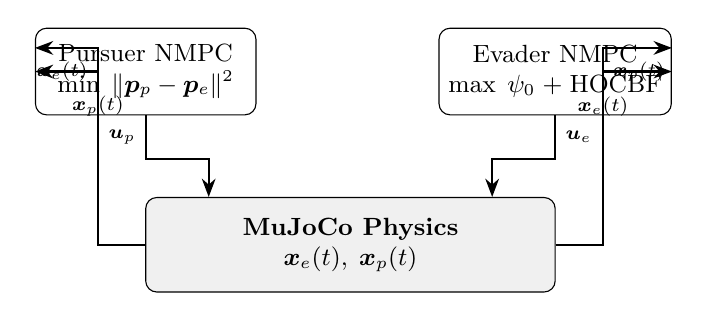
\begin{tikzpicture}[
    box/.style  = {draw, rounded corners, minimum width=2.8cm,
                   minimum height=1.1cm, align=center, font=\small},
    mujoco/.style = {draw, rounded corners, fill=gray!12,
                    minimum width=5.2cm, minimum height=1.2cm,
                    align=center, font=\small\bfseries},
    arr/.style  = {-Stealth, thick},
]
\node[mujoco]  (sim) at (0,0)   {MuJoCo Physics\\$\vect{x}_e(t),\;\vect{x}_p(t)$};
\node[box]     (pur) at (-2.6, 2.2) {Pursuer NMPC\\$\min\;\|\vect{p}_p-\vect{p}_e\|^2$};
\node[box]     (eva) at ( 2.6, 2.2) {Evader NMPC\\$\max\;\psi_0\;$+\;HOCBF};
\draw[arr] (sim.west)  -- ++(-0.6,0) |- node[left, font=\scriptsize]{$\vect{x}_e(t)$} (pur.west);
\draw[arr] (sim.east)  -- ++(+0.6,0) |- node[right,font=\scriptsize]{$\vect{x}_p(t)$} (eva.east);
\draw[arr] (pur.south) -- node[left, font=\scriptsize]{$\vect{u}_p$} ++(0,-0.55)
           -| ([xshift=-1.8cm]sim.north);
\draw[arr] (eva.south) -- node[right,font=\scriptsize]{$\vect{u}_e$} ++(0,-0.55)
           -| ([xshift=+1.8cm]sim.north);
\draw[arr] (sim.west)  -- ++(-0.6,0) |- node[pos=0.3,above,font=\scriptsize]{$\vect{x}_p(t)$}
           ([yshift=0.3cm]pur.west);
\draw[arr] (sim.east)  -- ++(+0.6,0) |- node[pos=0.3,above,font=\scriptsize]{$\vect{x}_e(t)$}
           ([yshift=0.3cm]eva.east);
\end{tikzpicture}
\caption{Closed-loop decoupled architecture.
         Each agent measures the other's current state and solves
         its own OCP independently at \SI{100}{\hertz}.}
\label{fig:architecture}
\end{figure}

% ── IV-B ──────────────────────────────────────────────────────────────────
\subsection{Augmented State for the Evader OCP}
\label{sec:aug_state}

To express $\psi_0$ and $\psi_1$ as explicit functions of the OCP
state (required by acados for the stage constraints), we
\emph{augment} the evader's state with the pursuer's predicted
position and velocity:
\begin{equation}
    \vect{z} =
    \begin{bmatrix}
        \vect{x}_e \\ \hat{\vect{p}}_p \\ \hat{\vect{v}}_p
    \end{bmatrix}
    \in \R^{19},
    \qquad
    \dot{\vect{z}} = \begin{bmatrix}
        f(\vect{x}_e, \vect{u}_e) \\
        \hat{\vect{v}}_p \\ \vect{0}_3
    \end{bmatrix},
    \label{eq:aug_state}
\end{equation}
where the constant-velocity
dynamics~\eqref{eq:pred_p}--\eqref{eq:pred_v} are embedded directly
in the OCP.
At each control step $t_k$, the initial conditions are set
as $\hat{\vect{p}}_p(0) = \vect{p}_p(t_k)$ and
$\hat{\vect{v}}_p(0) = \vect{v}_p(t_k)$
from the state estimate~\eqref{eq:ocp_ic}.

With this augmentation, the barrier functions become
\begin{align}
    \psi_0(\vect{z}) &= \norm{\vect{p}_e - \hat{\vect{p}}_p}^2
                        - d_{\min}^2,
                        \label{eq:psi0_aug} \\
    \psi_1(\vect{z}) &= 2\,(\vect{p}_e-\hat{\vect{p}}_p)^\top
                         (\vect{v}_e-\hat{\vect{v}}_p)
                         + \gamma_1\,\psi_0(\vect{z}),
                        \label{eq:psi1_aug}
\end{align}
which are purely functions of the OCP state $\vect{z}$ and require
no external parameters.

% ── IV-C ──────────────────────────────────────────────────────────────────
\subsection{Evader OCP: HOCBF Constraints in acados}
\label{sec:evader_ocp}

The evader's OCP is solved at \SI{100}{\hertz} using the
acados~\cite{verschueren2022acados} SQP-RTI solver with
Explicit Runge-Kutta (ERK4) integration and
\texttt{FULL\_CONDENSING\_HPIPM} as the inner QP solver.
The prediction horizon is $N=50$ steps at $\Delta t = \SI{10}{\milli\second}$
($T_H = \SI{0.5}{\second}$).

\subsubsection*{Nonlinear stage constraints}
Three nonlinear inequality constraints are imposed at every stage
$k\in\{0,\ldots,N-1\}$, expressed as
$\vect{h}(\vect{z}(k),\vect{u}(k)) \geq \vect{0}$
via \texttt{con\_h\_expr} in acados:
\begin{equation}
\vect{h}(\vect{z},\vect{u}) =
\begin{bmatrix}
    \psi_0(\vect{z}) \\[3pt]
    \psi_1(\vect{z}) \\[3pt]
    \lambda(\vect{z})\,T + \Phi(\vect{z}) + \gamma_2\,\psi_1(\vect{z})
\end{bmatrix}
\;\geq\;
\begin{bmatrix}0\\0\\0\end{bmatrix},
\label{eq:con_h}
\end{equation}
where $\lambda$ and $\Phi$ are given by~\eqref{eq:lambda}
and~\eqref{eq:Phi}, respectively.
Constraint~1 enforces minimum separation;
Constraint~2 prevents the velocity from driving the agents together
faster than the decay rate $\gamma_1$ allows;
Constraint~3 is the HOCBF rate condition~\eqref{eq:hocbf_affine},
which is \emph{affine in~$T$} and encodes the actual control authority.
The same constraints~1 and~2 are imposed at the terminal stage $N$
(no Constraint~3 at terminal since there is no $\vect{u}(N)$).

\subsubsection*{Input constraints}
Box constraints are imposed on all four inputs:
\begin{equation}
    T \in [T_{\min},\,T_{\max}],\quad
    \omega_j^{\mathrm{cmd}} \in [-\omega_{\max},\,\omega_{\max}],
    \quad j=x,y,z.
    \label{eq:input_box}
\end{equation}
Numerical values are given in Table~\ref{tab:params}.

\subsubsection*{Evasion cost}
The stage cost directly maximizes the squared separation:
\begin{equation}
    \ell(\vect{z},\vect{u})
        = -\beta\,\psi_0(\vect{z})
          + \vect{u}^\top \mat{R}\,\vect{u},
    \label{eq:stage_cost}
\end{equation}
with $\mat{R} = \mathrm{diag}(R_T,\,R_\omega\,\mat{I}_3)$.
The terminal cost $V_f = -\beta_N\,\psi_0(\vect{z}(N))$ provides
a consistent terminal incentive for maintaining distance.

% ── IV-D ──────────────────────────────────────────────────────────────────
\subsection{Pursuer OCP}
\label{sec:pursuer_ocp}

The pursuer runs a standard NMPC with the same body-rate model
(state $\vect{x}_p \in \R^{13}$, input $\vect{u}_p \in \R^4$)
and the same solver configuration (SQP-RTI, ERK4, $N=50$,
$\Delta t=\SI{10}{\milli\second}$).
At each step, the evader's current state $\vect{x}_e(t_k)$ is set
as the reference trajectory for the next $N$ steps (constant
reference assumption), and the pursuer minimizes
\begin{equation}
    \ell_p(\vect{x}_p,\vect{u}_p)
        = \norm{\vect{p}_p - \vect{p}_e}^2_{\mat{Q}_p}
          + \norm{\log(\vect{q}_p \ominus \vect{q}_e)}^2_{\mat{K}_p}
          + \vect{u}_p^\top \mat{R}_p\,\vect{u}_p,
    \label{eq:pursuer_cost}
\end{equation}
with diagonal weight matrices $\mat{Q}_p$, $\mat{K}_p$, $\mat{R}_p$.
No CBF constraints are imposed on the pursuer; it acts as a
worst-case adversary within its physical limits.

% ── IV-E ──────────────────────────────────────────────────────────────────
\subsection{Software Architecture}
\label{sec:software}

\subsubsection*{MiL stage (internal validation)}
Before connecting to MuJoCo, both agents are validated in a
Model-in-the-Loop (MiL) loop: the plant is the same quadrotor ODE
integrated with a fixed-step RK4 scheme in Python.
This stage verifies solver convergence, HOCBF constraint satisfaction,
and correct gain tuning without the overhead of the physics engine.

\subsubsection*{SiL stage (reported experiments)}
The final experiments use MuJoCo~3~\cite{todorov2012mujoco} as the
physics back-end.
Two independent ROS~2 (Humble) nodes,
\texttt{/drone\_evader} and \texttt{/drone\_pursuer},
each run one acados solver and publish body-rate commands at
\SI{100}{\hertz}.
The MuJoCo scene contains two identical quadrotor rigid bodies with
contact geometry; a drone-to-drone collision is therefore physically
detectable as a contact event, providing a ground-truth oracle for
constraint violation that RK4 integration cannot reproduce.
State observations are shared via zero-copy intra-process topics.
All acados solvers are code-generated from CasADi symbolic expressions
and compiled to C with Cython bindings.

Table~\ref{tab:params} summarizes the tuning parameters used
in all experiments.

\begin{table}[t]
\caption{Simulation and NMPC parameters.}
\label{tab:params}
\centering
\renewcommand{\arraystretch}{1.2}
\begin{tabular}{@{}llc@{}}
\toprule
\textbf{Parameter} & \textbf{Symbol} & \textbf{Value} \\
\midrule
Vehicle mass       & $m$             & \SI{1.08}{\kilo\gram} \\
Gravity            & $g$             & \SI{9.81}{\meter\per\second\squared} \\
Rate constant      & $\tau_{\mathrm{rc}}$ & \SI{30}{\milli\second} \\
Max thrust         & $T_{\max}$      & $3\,mg$ \\
Min thrust         & $T_{\min}$      & $0$ \\
Max angular rate   & $\omega_{\max}$ & \SI{3}{\radian\per\second} \\
Horizon steps      & $N$             & 50 \\
Sampling time      & $\Delta t$      & \SI{10}{\milli\second} \\
\midrule
Evasion weight     & $\beta,\beta_N$ & TBD \\
HOCBF decay-0      & $\gamma_1$      & TBD \\
HOCBF decay-1      & $\gamma_2$      & TBD \\
Min separation     & $d_{\min}$      & \SI{0.5}{\meter} \\
Pursuer accel.\ bound & $a_p^{\max}$ & \SI{2}{\meter\per\second\squared} \\
\bottomrule
\end{tabular}
\end{table}

% ═══════════════════════ V. RESULTS ══════════════════════
\section{Software-in-the-Loop Experiments}
\label{sec:results}

% TODO: MuJoCo SiL — three scenarios (free, cornering, speed-advantage)
% Metrics: violation rate, min separation, evasion distance, solve time
% Comparison: NMPC+HOCBF vs. CBF-QP post-hoc vs. NMPC without CBF

% ═══════════════════════ VI. CONCLUSION ══════════════════
\section{Conclusion}
\label{sec:conclusion}

% TODO: summary, limitations, future work

% ═══════════════════════ REFERENCES ══════════════════════
\bibliographystyle{IEEEtran}

\begin{thebibliography}{30}

% ── Pursuit-evasion: RL / MARL ─────────────────────────
\bibitem{wang2022game}
H.~Wang, W.~Lyu, and P.~Yao,
``Game of drones: Multi-UAV pursuit-evasion game with online motion planning
  by deep reinforcement learning,''
\emph{IEEE Transactions on Neural Networks and Learning Systems},
vol.~34, no.~12, pp.~10,592--10,603, 2023.

\bibitem{zhang2024online}
J.~Zhang \emph{et~al.},
``Online planning for multi-UAV pursuit-evasion in unknown environments by
  deep reinforcement learning,''
\emph{IEEE Robotics and Automation Letters},
vol.~9, no.~12, pp.~10,951--10,958, 2024.

\bibitem{lin2025adaptive}
Z.~Lin \emph{et~al.},
``Adaptive teaming in multi-drone pursuit: Simulation, training, and
  deployment,''
\emph{arXiv preprint arXiv:2502.09762}, 2025.

\bibitem{gu2024learning}
Y.~Gu \emph{et~al.},
``Learning multi-pursuit evasion for safe targeted navigation of drones,''
\emph{IEEE Robotics and Automation Letters},
vol.~9, no.~7, pp.~6,197--6,204, 2024.

\bibitem{kaufmann2025learned}
E.~Kaufmann \emph{et~al.},
``Learned controllers for agile quadrotors in pursuit-evasion games,''
\emph{arXiv preprint arXiv:2506.02849}, 2025.

% ── Pursuit-evasion: MPC / game theory ────────────────
\bibitem{selvakumar2021pursuit}
J.~Selvakumar and E.~Bakolas,
``Pursuit-evasion games based on game-theoretic and MPC algorithms,''
in \emph{Proc.\ IEEE Conference on Decision and Control (CDC)},
2021, pp.~1--6.

\bibitem{belinha2024noncooperative}
R.~Belinha \emph{et~al.},
``Non-cooperative model predictive control for capturing a remotely piloted
  target drone,''
in \emph{Proc.\ ROBOT 2023: Sixth Iberian Robotics Conference},
Springer, 2024, pp.~1--12.

\bibitem{zhan2025nonlinear}
Y.~Zhan \emph{et~al.},
``Nonlinear receding-horizon differential game for drone racing,''
\emph{arXiv preprint arXiv:2502.01044}, 2025.

\bibitem{zeng2024decentralized}
J.~Zeng \emph{et~al.},
``Decentralized nonlinear model predictive control for safe collision
  avoidance in quadrotor teams with exponential control barrier functions,''
\emph{arXiv preprint arXiv:2409.17379}, 2024.

% ── Pursuit-evasion: CBF on pursuer / hybrid ──────────
\bibitem{chu2024control}
Y.~Chu \emph{et~al.},
``Control barrier function-based collision avoidance guidance for
  multi-fixed-wing UAV pursuit-evasion,''
\emph{Drones}, vol.~8, no.~8, p.~415, 2024.

\bibitem{zhou2025control}
X.~Zhou, N.~Atanasov \emph{et~al.},
``Control strategies for pursuit-evasion under occlusion using visibility
  and safety barrier functions,''
in \emph{Proc.\ IEEE International Conference on Robotics and
  Automation (ICRA)}, 2025.

\bibitem{zhang2025embedded}
K.~Zhang \emph{et~al.},
``Embedded safe reactive navigation for multirotors using control barrier
  functions,''
in \emph{Proc.\ International Conference on Unmanned Aircraft Systems
  (ICUAS)}, 2025.

% ── CBF theory ────────────────────────────────────────
\bibitem{ames2019control}
A.~D.~Ames, S.~Coogan, M.~Egerstedt, G.~Notomista, K.~Sreenath,
  and P.~Tabuada,
``Control barrier functions: Theory and applications,''
in \emph{Proc.\ European Control Conference (ECC)}, 2019, pp.~3420--3431.

\bibitem{xiao2021high}
W.~Xiao and C.~Belta,
``High-order control barrier functions,''
\emph{IEEE Transactions on Automatic Control},
vol.~67, no.~7, pp.~3655--3662, 2022.

\bibitem{liu2023iterative}
Z.~Liu, J.~Zeng, K.~Sreenath, and C.~Belta,
``Iterative convex optimization for model predictive control with
  discrete-time high-order control barrier functions,''
in \emph{Proc.\ American Control Conference (ACC)}, 2023, pp.~3368--3375.

\bibitem{zeng2021safety}
J.~Zeng, B.~Zhang, and K.~Sreenath,
``Safety-critical model predictive control with discrete-time control
  barrier functions,''
in \emph{Proc.\ American Control Conference (ACC)}, 2021, pp.~3882--3889.

\bibitem{zeng2021enhancing}
J.~Zeng, Z.~Li, and K.~Sreenath,
``Enhancing feasibility and safety of nonlinear model predictive control
  with discrete-time control barrier functions,''
in \emph{Proc.\ IEEE Conference on Decision and Control (CDC)},
2021, pp.~6137--6144.

\bibitem{zhu2025exponential}
M.~Zhu \emph{et~al.},
``Exponential control barrier functions and model predictive control for
  jerk-level reactive motion planning of quadrotors,''
\emph{Control Engineering Practice}, vol.~158, 2025.

% ── Drone dynamics / control ───────────────────────────
\bibitem{mellinger2011minimum}
D.~Mellinger and V.~Kumar,
``Minimum snap trajectory generation and control for quadrotors,''
in \emph{Proc.\ IEEE International Conference on Robotics and
  Automation (ICRA)}, 2011, pp.~2520--2525.

\bibitem{mueller2015model}
M.~W.~Mueller and R.~D'Andrea,
``A model predictive controller for quadrocopter state interception,''
in \emph{Proc.\ European Control Conference (ECC)}, 2013, pp.~1--8.

\bibitem{lee2010geometric}
T.~Lee, M.~Leok, and N.~H.~McClamroch,
``Geometric tracking control of a quadrotor UAV on SE(3),''
in \emph{Proc.\ IEEE Conference on Decision and Control (CDC)},
2010, pp.~5420--5425.

\bibitem{todorov2012mujoco}
E.~Todorov, T.~Erez, and Y.~Tassa,
``MuJoCo: A physics engine for model-based control,''
in \emph{Proc.\ IEEE/RSJ International Conference on Intelligent
  Robots and Systems (IROS)}, 2012, pp.~5026--5033.

% ── Solvers / framework ───────────────────────────────
\bibitem{verschueren2022acados}
R.~Verschueren \emph{et~al.},
``acados---A modular open-source framework for fast embedded
  optimal control,''
\emph{Mathematical Programming Computation},
vol.~14, pp.~147--183, 2022.

\bibitem{diehl2005real}
M.~Diehl, H.~G.~Bock, and J.~P.~Schl\"{o}der,
``A real-time iteration scheme for nonlinear optimization in optimal
  feedback control,''
\emph{SIAM Journal on Control and Optimization},
vol.~43, no.~5, pp.~1714--1736, 2005.

% ── Game theory ───────────────────────────────────────
\bibitem{isaacs1965differential}
R.~Isaacs,
\emph{Differential Games}.
John Wiley \& Sons, 1965.

\bibitem{shaferman2008cooperative}
V.~Shaferman and T.~Shima,
``Cooperative multiple model adaptive pursuit guidance,''
\emph{Journal of Guidance, Control, and Dynamics},
vol.~31, no.~4, pp.~1158--1167, 2008.

\end{thebibliography}

\vfill

\end{document}
